% Options for packages loaded elsewhere
\PassOptionsToPackage{unicode}{hyperref}
\PassOptionsToPackage{hyphens}{url}
\PassOptionsToPackage{dvipsnames,svgnames,x11names}{xcolor}
%
\documentclass[
  10pt,
]{article}
\usepackage{amsmath,amssymb}
\usepackage{iftex}
\ifPDFTeX
  \usepackage[T1]{fontenc}
  \usepackage[utf8]{inputenc}
  \usepackage{textcomp} % provide euro and other symbols
\else % if luatex or xetex
  \usepackage{unicode-math} % this also loads fontspec
  \defaultfontfeatures{Scale=MatchLowercase}
  \defaultfontfeatures[\rmfamily]{Ligatures=TeX,Scale=1}
\fi
\usepackage{lmodern}
\ifPDFTeX\else
  % xetex/luatex font selection
  \setmainfont[]{Times New Roman}
  \setmonofont[]{Menlo}
\fi
% Use upquote if available, for straight quotes in verbatim environments
\IfFileExists{upquote.sty}{\usepackage{upquote}}{}
\IfFileExists{microtype.sty}{% use microtype if available
  \usepackage[]{microtype}
  \UseMicrotypeSet[protrusion]{basicmath} % disable protrusion for tt fonts
}{}
\makeatletter
\@ifundefined{KOMAClassName}{% if non-KOMA class
  \IfFileExists{parskip.sty}{%
    \usepackage{parskip}
  }{% else
    \setlength{\parindent}{0pt}
    \setlength{\parskip}{6pt plus 2pt minus 1pt}}
}{% if KOMA class
  \KOMAoptions{parskip=half}}
\makeatother
\usepackage{xcolor}
\usepackage[margin=1in]{geometry}
\usepackage{longtable,booktabs,array}
\usepackage{calc} % for calculating minipage widths
% Correct order of tables after \paragraph or \subparagraph
\usepackage{etoolbox}
\makeatletter
\patchcmd\longtable{\par}{\if@noskipsec\mbox{}\fi\par}{}{}
\makeatother
% Allow footnotes in longtable head/foot
\IfFileExists{footnotehyper.sty}{\usepackage{footnotehyper}}{\usepackage{footnote}}
\makesavenoteenv{longtable}
\usepackage{graphicx}
\makeatletter
\def\maxwidth{\ifdim\Gin@nat@width>\linewidth\linewidth\else\Gin@nat@width\fi}
\def\maxheight{\ifdim\Gin@nat@height>\textheight\textheight\else\Gin@nat@height\fi}
\makeatother
% Scale images if necessary, so that they will not overflow the page
% margins by default, and it is still possible to overwrite the defaults
% using explicit options in \includegraphics[width, height, ...]{}
\setkeys{Gin}{width=\maxwidth,height=\maxheight,keepaspectratio}
% Set default figure placement to htbp
\makeatletter
\def\fps@figure{htbp}
\makeatother
\setlength{\emergencystretch}{3em} % prevent overfull lines
\providecommand{\tightlist}{%
  \setlength{\itemsep}{0pt}\setlength{\parskip}{0pt}}
\setcounter{secnumdepth}{-\maxdimen} % remove section numbering
\ifLuaTeX
  \usepackage{selnolig}  % disable illegal ligatures
\fi
\IfFileExists{bookmark.sty}{\usepackage{bookmark}}{\usepackage{hyperref}}
\IfFileExists{xurl.sty}{\usepackage{xurl}}{} % add URL line breaks if available
\urlstyle{same}
\hypersetup{
  pdftitle={What linear emotion probes on LLM hidden states do and do not buy you: an audit},
  pdfauthor={Justin Van Wart},
  colorlinks=true,
  linkcolor={Maroon},
  filecolor={Maroon},
  citecolor={Blue},
  urlcolor={Blue},
  pdfcreator={LaTeX via pandoc}}

\title{What linear emotion probes on LLM hidden states do and do not buy
you: an audit}
\author{Justin Van Wart}
\date{2026}

\begin{document}
\maketitle

{
\hypersetup{linkcolor=}
\setcounter{tocdepth}{2}
\tableofcontents
}
\hypertarget{abstract}{%
\subsection{Abstract}\label{abstract}}

Linear emotion probes read emotion-concept directions from a language
model\textquotesingle s residual stream and are a common basis for
visualisations and proposed monitors. We audit them on three small open
models (Llama-3.2-3B, Gemma-2-2B, Mistral-7B; 4-bit) against baselines
trained on the same data, using a frozen, hash-verified human test set
(GoEmotions, n=840), three further human-labelled sources,
pre-registered decision rules and paired bootstrap intervals. In-domain,
TF-IDF beats the probe by 0.09--0.13 macro-F1 on all three models.
Across domains the probe beats TF-IDF on every external source, but not
a frozen 110M-parameter sentence encoder, which ties or wins in every
model--source cell. Probes trained only on LLM-written text, the usual
recipe, reach about 0.31 macro-F1 on human text against 0.55--0.59 with
human training data, and a published 205,200-story model-written corpus
is lexically solvable (TF-IDF 0.930 vs probe 0.861). Probe z-scores
depend strongly on text length; with a threshold set on LLM-written text
the probe labels 56--81\% of neutral human text as emotional, and a
human-calibrated threshold restores neutral recall at a cost of
0.13--0.17 macro-F1. Adding probe directions to the residual stream
changed expressed emotion beyond random controls for 0 of 7 emotions on
Llama and 4 of 7, a threshold pass, on Gemma. We release the audit tool,
test-set manifests and all pre-registrations.

\hypertarget{1-question-position-and-design}{%
\subsection{1. Question, position and
design}\label{1-question-position-and-design}}

\hypertarget{11-why-audit}{%
\subsubsection{1.1 Why audit}\label{11-why-audit}}

Emotion probes are usually built from LLM-generated emotional passages
and then shown to separate held-out passages from the same generator.
That is weak evidence: such corpora can be lexically solvable. Our first
corpus was exactly that: TF-IDF reached macro-F1 0.931 {[}0.906,
0.953{]} (topic-disjoint, 3 seeds;
\texttt{data/corpus/corpus\_v1\_tfidf\_gate.md}) against 0.857 for the
probe (\texttt{docs/FINDINGS.md}; the two numbers come from different
splits). The interpretability literature has known since control tasks
were introduced (Hewitt \& Liang, 2019) that probe accuracy means little
without baselines. Emotion-probe studies rarely include them.

\hypertarget{12-position-relative-to-recent-work}{%
\subsubsection{1.2 Position relative to recent
work}\label{12-position-relative-to-recent-work}}

Sofroniew et al. (2026) extracted 171 emotion-concept vectors from
Claude Sonnet 4.5 using model-written stories and showed that they
influence behaviour. Several studies replicated the representational
part on open models with model-generated corpora (van der Ben et al.,
2026; Hollowell, 2026; Jeong, 2026a,b). Reichman et al. (2026) report an
emotional subspace, found from a synthetic rewritten-sentence dataset,
whose probes generalise across eight real datasets and five languages.
Fang et al. (2026) probe eight 1B--9B open models, including
Llama-3.2-3B, on GoEmotions and two other corpora, and test transfer
across corpora. Zhang \& Zhong (2025) release a probing toolkit and a
Reddit emotion dataset. Keeman (2026) controls for keywords differently:
clinical vignettes with the emotion words removed, on six Llama and
Gemma models, where emotion categorisation drops 1--7\% without
keywords. For steering, activation addition (Turner et al., 2023) and
contrastive activation addition (Panickssery et al., 2023) add
mean-difference vectors to the residual stream, and Marks \& Tegmark
(2023) found for true/false statements that difference-in-means
directions are more causally implicated in model outputs than directions
from other probing techniques.

None of these compares the probe with a lexical or bag-of-embeddings
classifier trained on the same data, separates in-domain from
cross-domain evaluation against such baselines, or checks calibration on
neutral human text. Those comparisons are our contribution. We do not
claim novelty for linear emotion probing, for cross-domain transfer as
such, or for the valence geometry.

\hypertarget{13-contributions}{%
\subsubsection{1.3 Contributions}\label{13-contributions}}

\begin{enumerate}
\def\labelenumi{\arabic{enumi}.}
\tightlist
\item
  \textbf{An in-domain/cross-domain reversal, on three model families.}
  A lexical classifier beats the probe in-domain; the probe beats it
  across domains. The probe does not beat a frozen sentence encoder
  trained on the same data (H3 not supported): it ties on dair and on
  the in-domain set and loses on ISEAR and DailyDialog for all three
  models, so the cross-domain advantage over lexical models is not
  specific to LLM probes.
\item
  \textbf{A cost for the common recipe.} Probes built only from
  LLM-written emotional text transfer weakly to human text, and
  LLM-written data add nothing once human data are present.
\item
  \textbf{Calibration and neutral detection fail.} Raw z-scores depend
  strongly on text length, and recalibration does not meet
  pre-registered bounds. This matters for any live display or monitor.
\item
  \textbf{Reading does not guarantee writing, and it is
  model-dependent.} Adding the audited probe directions to the residual
  stream does not change the emotion Llama-3.2-3B expresses beyond
  random directions (0 of 7, pre-registered), but does on Gemma-2-2B for
  4 of 7 emotions at the largest fluent strength (pre-registered
  replication, H7a). A fluency-matched Llama re-run again gives 0 of 7.
  Mean-difference directions are not better than probe directions at
  matched fluency (H7b, H8b not established); on Gemma this holds when
  both are fitted on the same data (H9, 0 of 7), while on Llama the two
  were fitted on different corpora.
\item
  \textbf{A model-written corpus is a weak yardstick (audit of a
  published corpus).} On a subsample of a published 205,200-story
  Gemini-written corpus, TF-IDF (0.930) beats the probe (0.861)
  in-corpus; a probe trained on it transfers to human text above
  same-data TF-IDF but at 0.21--0.45 macro-F1, and a probe trained on
  our corpus loses 0.319 on its held-out stories (section 2.9).
\item
  \textbf{A reusable audit tool} (\texttt{probekit\ audit}) with frozen,
  hash-verified human test sets and fetch scripts.
\end{enumerate}

\hypertarget{14-design}{%
\subsubsection{1.4 Design}\label{14-design}}

\textbf{Baselines.} Each comparison trains the baseline on the same data
as the probe:

\begin{itemize}
\tightlist
\item
  (a) TF-IDF + logistic regression;
\item
  (b) NRC EmoLex word counts (Mohammad \& Turney, 2013), no training.
  This separates "lexical features fail across domains" from "features
  fitted to the training domain fail";
\item
  (c) logistic regression on the mean of the model\textquotesingle s
  input token embeddings ("bag of embeddings": vocabulary knowledge, no
  context);
\item
  (d) a frozen pretrained sentence encoder + logistic regression.
  \texttt{sentence-transformers/all-mpnet-base-v2} (revision
  e8c3b32edf5434bc2275fc9bab85f82640a19130, 109.5M parameters, 768
  dimensions; sentence-transformers library, Reimers \& Gurevych, 2019).
  The encoder is frozen; a logistic regression (StandardScaler, C on
  validation) is trained on its embeddings with the same recipe as the
  native-LR baseline. The model card lists Reddit comments (2015--2018;
  726M of its more than 1B training pairs) among the
  encoder\textquotesingle s training data, so it may have seen text from
  the same domain as GoEmotions; this bears more on the in-domain
  comparison than on the external sources;
\item
  (e) logistic regression on the same hidden states as the probe (the
  linear ceiling);
\item
  (f) a shuffled-label null.
\end{itemize}

Comparisons are paired over the same test items and reported with
bootstrap 95\% intervals. Headline comparisons are also repeated over 5
training seeds or subsamples (section 2.7).

\textbf{Pre-registered hypotheses.} H1: probe − TF-IDF \textgreater{} 0
cross-domain (CI above 0 on ≥ 2 of 3 sources). H2: probe − bag of
embeddings \textgreater{} 0. H3 (added before the run,
\texttt{0d74f80}): probe − sentence encoder \textgreater{} 0, CI above 0
on ≥ 2 of 3 external sources per model, on ≥ 2 of 3 models. If H3 fails,
we report the encoder as equivalent or better and do not claim
LLM-specific information. \textbf{H3 failed} (section 2.2). H4 (EmoLex,
descriptive), H5 (human-neutral threshold, rule in 2.6) and H6 (five
training seeds) were pre-registered in the same commit. D2: native LR at
k=378 − k=80 \textgreater{} 0.03 means data-limited.

\textbf{Probes.} One direction per emotion (joy, sadness, fear, anger,
surprise, disgust, love), fitted by shrinkage LDA, logistic regression
or mean difference on mean-pooled mid-layer states (first 4 tokens
skipped). Scores are z-scored against held-out neutral text, with a
neutral threshold τ. Layer, estimator and τ are chosen on validation
only. The extractor uses a causal mask and is checked against each
model\textquotesingle s own forward pass (relative difference 3e-4 to
6e-4); it handles Gemma\textquotesingle s embedding scaling.

\textbf{Data.} Training: LLM-written passages from two writers
(Llama-3.2-3B and Qwen3.8-27B) plus human GoEmotions comments (up to 378
per class, official train split only). Test:

\begin{itemize}
\tightlist
\item
  (i) a frozen GoEmotions test set: official test split, single-label
  items, near-duplicates of train/dev removed, n=840, 63--151 per class,
  SHA-256 manifest; the evaluator refuses a modified file
  {[}\texttt{data/testsets/*.manifest.json}{]};
\item
  (ii) dair-ai/emotion test (tweets, hashtag-derived labels; Saravia et
  al., 2018), ISEAR (first-person event descriptions; Scherer \&
  Wallbott, 1994) and DailyDialog (utterances; Li et al., 2017). The
  GoEmotions set is Demszky et al. (2020).
\end{itemize}

Class sets differ across sources, so predictions are restricted to each
source\textquotesingle s classes. Calm exists only in LLM-written text
(confounded with writer) and is excluded from all headline numbers.

\textbf{Models.} Llama-3.2-3B-Instruct, Gemma-2-2B-it and
Mistral-7B-Instruct, all 4-bit via MLX. The Mistral model is
Mistral-7B-Instruct-v0.3
(\texttt{mlx-community/Mistral-7B-Instruct-v0.3-4bit}). Mistral was
chosen as a third family at the largest size that runs comfortably on
the hardware used; it is an older model, and results may differ on newer
7--9B models.

\hypertarget{2-results}{%
\subsection{2. Results}\label{2-results}}

\textbf{Figure 1} (\texttt{docs/figures/fig1\_forest.svg};
\texttt{make\_figures.py}; data \texttt{t11.json},
\texttt{external\_eval.json}). Forest plot: probe − baseline (TF-IDF,
sentence encoder, bag of embeddings), macro-F1 with 95\% CI. Rows:
frozen in-domain set (shaded) plus three external sources; panels: three
models; a vertical line at 0. All systems are trained on the HUM set
(LLM-written rows plus the human pool); the in-domain bag-of-embeddings
difference is post hoc (\texttt{t11\_posthoc.json}). This figure carries
the paper.

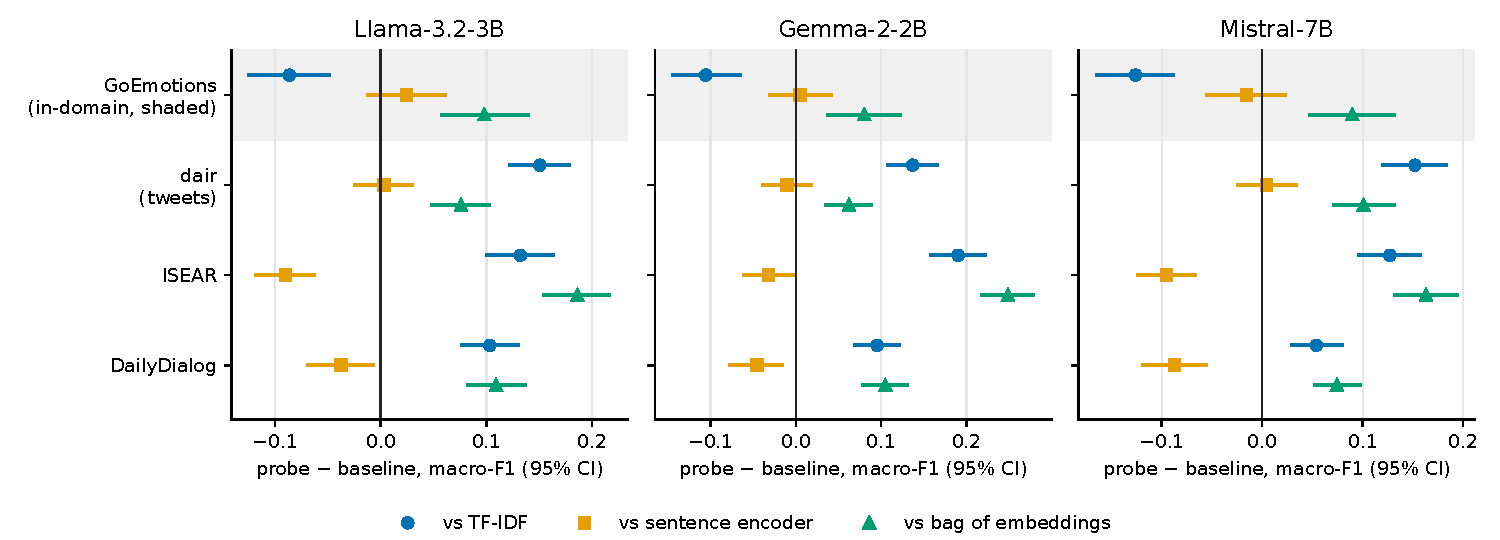
\includegraphics{../figures/fig1_forest.pdf}

\hypertarget{21-in-domain-lexical-features-win-t11md-t11_posthocmd}{%
\subsubsection{\texorpdfstring{2.1 In-domain, lexical features win
{[}\texttt{t11.md},
\texttt{t11\_posthoc.md}{]}}{2.1 In-domain, lexical features win {[}t11.md, t11\_posthoc.md{]}}}\label{21-in-domain-lexical-features-win-t11md-t11_posthocmd}}

On the GoEmotions frozen set (8-way, chance 0.125), every system trained
on the same HUM data (LLM-written rows plus the human GoEmotions-train
pool, n=4,192). HUM is the training set for all comparisons in 2.1--2.7
and for Figure 1; the first pre-registered run, on a different training
set, is Appendix A and reaches the same conclusion.

\begin{longtable}[]{@{}llll@{}}
\toprule\noalign{}
system & Llama-3.2-3B & Gemma-2-2B & Mistral-7B \\
\midrule\noalign{}
\endhead
\bottomrule\noalign{}
\endlastfoot
probe & 0.587 {[}0.554, 0.619{]} & 0.568 {[}0.534, 0.600{]} & 0.549
{[}0.513, 0.580{]} \\
trained classifier, same states & 0.641 {[}0.606, 0.670{]} & 0.634
{[}0.598, 0.666{]} & 0.653 {[}0.618, 0.683{]} \\
TF-IDF & 0.674 {[}0.640, 0.704{]} & 0.674 {[}0.640, 0.704{]} & 0.674
{[}0.640, 0.704{]} \\
sentence encoder & 0.563 {[}0.527, 0.594{]} & 0.563 {[}0.527, 0.594{]} &
0.563 {[}0.527, 0.594{]} \\
bag of embeddings & 0.489 & 0.488 & 0.458 \\
EmoLex (no training) & 0.248 {[}0.213, 0.278{]} & 0.248 {[}0.213,
0.278{]} & 0.248 {[}0.213, 0.278{]} \\
probe − TF-IDF & −0.086 {[}−0.124, −0.049{]} & −0.106 {[}−0.144,
−0.065{]} & −0.126 {[}−0.165, −0.088{]} \\
probe − sentence encoder (H3) & +0.024 {[}−0.012, +0.061{]} & +0.005
{[}−0.031, +0.042{]} & −0.015 {[}−0.055, +0.023{]} \\
probe − EmoLex (H4) & +0.339 {[}+0.294, +0.384{]} & +0.320 {[}+0.276,
+0.364{]} & +0.300 {[}+0.254, +0.344{]} \\
probe − bag of embeddings (H2; post hoc on HUM) & +0.098 {[}+0.058,
+0.139{]} & +0.080 {[}+0.038, +0.122{]} & +0.090 {[}+0.048, +0.132{]} \\
probe − trained classifier (post hoc) & −0.053 {[}−0.081, −0.026{]} &
−0.066 {[}−0.095, −0.037{]} & −0.106 {[}−0.133, −0.080{]} \\
\end{longtable}

{[}\texttt{t11.md} and \texttt{t11\_posthoc.md} in each
model\textquotesingle s directory.{]} TF-IDF, EmoLex and the sentence
encoder do not use the LLM, so their rows are identical across models.
The probe sits between the bag of embeddings and the lexical and encoder
baselines. In-domain the probe and the sentence encoder are
indistinguishable (H3 concerns the external sources, 2.2), and the
trained classifier on the same states is above the probe on all three
models, so one direction per emotion leaves in-domain performance on the
table.

\hypertarget{22-across-domains-the-probe-beats-lexical-models-external_evalmd}{%
\subsubsection{\texorpdfstring{2.2 Across domains, the probe beats
lexical models
{[}\texttt{external\_eval.md}{]}}{2.2 Across domains, the probe beats lexical models {[}external\_eval.md{]}}}\label{22-across-domains-the-probe-beats-lexical-models-external_evalmd}}

Trained on the same GoEmotions-derived data and tested on other human
sources, probe − TF-IDF (macro-F1 {[}95\% CI{]}, H1):

\begin{itemize}
\tightlist
\item
  Llama: dair +0.151 {[}+0.122, +0.178{]}, ISEAR +0.132 {[}+0.101,
  +0.163{]}, DailyDialog +0.103 {[}+0.077, +0.130{]};
\item
  Gemma: +0.137, +0.190, +0.095;
\item
  Mistral: +0.152, +0.127, +0.054.
\end{itemize}

All intervals exclude 0. Trained only on LLM-written text, the gaps are
larger: Llama +0.167, +0.262, +0.125; Gemma +0.127, +0.264, +0.152;
Mistral +0.135, +0.196, +0.092.

Against the zero-training lexicon (H4, descriptive; all intervals
exclude 0 in the probe\textquotesingle s favour): Llama dair +0.133
{[}+0.106, +0.159{]}, ISEAR +0.251 {[}+0.219, +0.282{]}, DailyDialog
+0.118 {[}+0.083, +0.151{]}; Gemma +0.119, +0.309, +0.110; Mistral
+0.134, +0.246, +0.069 {[}+0.036, +0.100{]}. EmoLex scores 0.226--0.316
on the external sources and 0.248 on the frozen set: close to TF-IDF
trained on HUM on dair and DailyDialog (0.254, 0.240), below it on ISEAR
(0.434), and below the probe on every source.

Against the frozen sentence encoder (H3; probe − encoder, macro-F1
{[}95\% CI{]}, all trained on HUM; \texttt{t11.md}):

\begin{longtable}[]{@{}llll@{}}
\toprule\noalign{}
model & dair & ISEAR & DailyDialog \\
\midrule\noalign{}
\endhead
\bottomrule\noalign{}
\endlastfoot
Llama & +0.003 {[}−0.024, +0.030{]} & −0.090 {[}−0.118, −0.063{]} &
−0.038 {[}−0.069, −0.007{]} \\
Gemma & −0.011 {[}−0.038, +0.018{]} & −0.032 {[}−0.061, −0.004{]} &
−0.046 {[}−0.077, −0.017{]} \\
Mistral & +0.004 {[}−0.024, +0.034{]} & −0.095 {[}−0.123, −0.067{]} &
−0.087 {[}−0.118, −0.056{]} \\
\end{longtable}

The probe\textquotesingle s interval is above 0 on 0 of 3 sources for 0
of 3 models, so \textbf{H3 is not supported} (\texttt{t11\_summary.md}).
The encoder is better on ISEAR and DailyDialog for every model and tied
on dair. We therefore make no claim that the probes carry emotion
information beyond a generic sentence encoder.

\textbf{Hidden states versus the encoder (post hoc, not pre-registered;
\texttt{t11\_posthoc.md}).} H3 tested the single-direction probe. The
trained classifier on the same hidden states, native LR minus the
encoder (HUM training; paired bootstrap):

\begin{longtable}[]{@{}lllll@{}}
\toprule\noalign{}
model & frozen (in-domain) & dair & ISEAR & DailyDialog \\
\midrule\noalign{}
\endhead
\bottomrule\noalign{}
\endlastfoot
Llama & +0.078 {[}+0.043, +0.112{]} & +0.003 {[}−0.025, +0.030{]} &
−0.082 {[}−0.109, −0.054{]} & +0.029 {[}−0.003, +0.061{]} \\
Gemma & +0.071 {[}+0.035, +0.106{]} & +0.004 {[}−0.024, +0.032{]} &
−0.061 {[}−0.087, −0.035{]} & +0.053 {[}+0.018, +0.089{]} \\
Mistral & +0.091 {[}+0.053, +0.127{]} & +0.006 {[}−0.024, +0.037{]} &
−0.061 {[}−0.088, −0.034{]} & +0.018 {[}−0.012, +0.048{]} \\
\end{longtable}

In-domain the states carry more than the encoder (all three intervals
above 0). Across domains the classifier ties the encoder on dair, is
below it on ISEAR, and is at or above it on DailyDialog (above only for
Gemma). So the hidden states hold more in-domain information than the
encoder, but a single direction per emotion does not extract it, and the
cross-domain picture is mixed rather than a clear win for either. The H3
verdict for the probe is unchanged.

\textbf{Robustness to ISEAR (post hoc;
\texttt{t11\_leave\_one\_source\_out.md}).} ISEAR is the
weakest-provenance source (Hub copy, 5 classes) and the one where the
encoder\textquotesingle s lead is largest. Dropping it, H1 still holds
for all three models, and the probe still ties the encoder on dair and
loses to it on DailyDialog, so H3 stays unsupported; H1 holds and H3
fails under every single-source drop.

\emph{Reading.} Lexical models fit the vocabulary of their training
domain; contextual representations transfer better. The LLM probe is no
better at this than a frozen sentence encoder (and worse on two
sources), so the cross-domain advantage over lexical models is not
specific to these LLMs.

Caveats: one encoder only (a larger or emotion-fine-tuned encoder could
widen the gap); the encoder\textquotesingle s training data include
Reddit comments, so in-domain it may have seen text like GoEmotions (the
external sources are less affected); the encoder and the probe see the
same training rows but the encoder reads whole sentences with a model
built for sentence similarity; dair labels are hashtag-derived and
lexical; ISEAR provenance is unverified; sources differ in class sets.

\hypertarget{23-llm-written-training-data-are-not-enough-human-data-are-the-lever-frozen_evalmd}{%
\subsubsection{\texorpdfstring{2.3 LLM-written training data are not
enough; human data are the lever
{[}\texttt{frozen\_eval.md}{]}}{2.3 LLM-written training data are not enough; human data are the lever {[}frozen\_eval.md{]}}}\label{23-llm-written-training-data-are-not-enough-human-data-are-the-lever-frozen_evalmd}}

\begin{itemize}
\tightlist
\item
  With \emph{no} human training data, the probes score 0.305--0.313 on
  the frozen human set (shuffle-null p95 ≈ 0.13); TF-IDF scores 0.146.
\item
  Adding human rows (0 → 378 per class) raises frozen-set F1 steadily:
  native LR at k=378 vs k=80 gives +0.069 {[}+0.039, +0.099{]} on Llama,
  +0.103 on Gemma and +0.096 on Mistral (D2: data-limited).
\item
  Once human data are present, LLM-written rows add nothing measurable:
  human-only training equals LLM + human at every k.
\item
  With full HUM training the trained classifier on the same states is
  above the probe in-domain on all three models (−0.053 to −0.106 for
  probe − classifier) and on DailyDialog (−0.067 to −0.105); it ties the
  probe on dair and is mixed on ISEAR (Gemma probe +0.029, Mistral
  −0.035; post hoc, \texttt{t11\_posthoc.md}). Restricting to a single
  direction per class therefore costs something where there is enough
  human data; the pre-registered nonlinear checks (2.4) still find
  nothing beyond a linear read-out.
\end{itemize}

\textbf{Figure 2} (\texttt{docs/figures/fig2\_learning\_curve.svg}; data
\texttt{frozen\_eval.json}). Learning curve: frozen-set macro-F1 against
human rows per class (0--378), probe / native LR / TF-IDF, LLM + human
vs human-only, mean ± sd over three subsampling seeds, three models; the
human-only curve starts at k=20. The k=378 point is a single fit without
seed variance, and the human-only curves dip there for Gemma and
Mistral; this is not an effect we interpret.

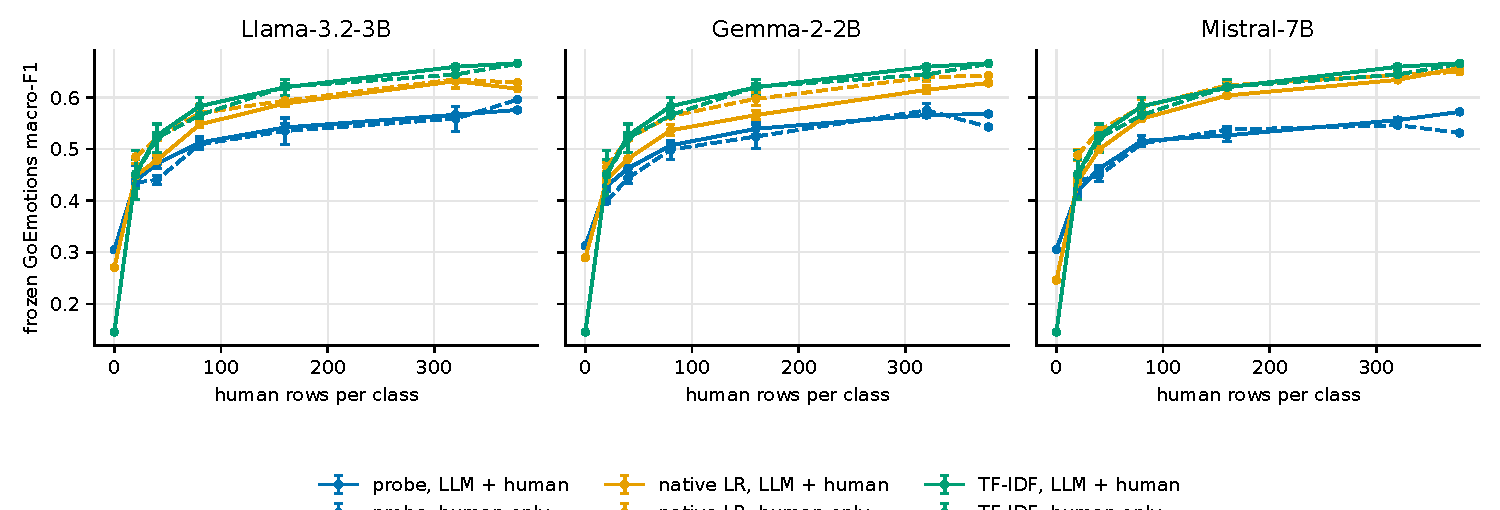
\includegraphics{../figures/fig2_learning_curve.pdf}

This bears on the common practice of building emotion vectors from
model-written stories (Sofroniew et al., 2026, and the replications in
1.2). Those studies target representational geometry and behaviour, not
classifying human text, so our result does not contradict them. It does
show that a probe built that way should not be assumed to read
human-written emotion well.

\hypertarget{24-linear-is-enough-geometry-is-human-like-on-two-models-t8_experimentsmd}{%
\subsubsection{\texorpdfstring{2.4 Linear is enough; geometry is
human-like on two models
{[}\texttt{t8\_experiments.md}{]}}{2.4 Linear is enough; geometry is human-like on two models {[}t8\_experiments.md{]}}}\label{24-linear-is-enough-geometry-is-human-like-on-two-models-t8_experimentsmd}}

\begin{itemize}
\tightlist
\item
  \textbf{Read-out.} A valence hierarchy beat flat logistic regression
  on at most 1 of 4 sets, and an MLP on 0 of 4 (rule: ≥ 3 of 4), on all
  three models.
\item
  \textbf{Geometry.} The 21 pairwise dissimilarities of the probe
  directions correlate with pairwise valence--arousal--dominance
  distances between the seven emotion words (NRC VAD v2.1; Mohammad,
  2025). Spearman ρ = +0.53 / +0.60 (Llama, lda / mean-diff) and +0.61 /
  +0.63 (Gemma), all p ≤ 0.016 under an exact permutation over 5040
  labelings. On Mistral the mean-difference directions agree (+0.54,
  p=0.005) but the validation-selected logreg directions do not (+0.31,
  p=0.112), so the pre-registered rule is not met there. Seven points;
  nominal.
\end{itemize}

\hypertarget{25-pooling-and-prompting-variantsmd}{%
\subsubsection{\texorpdfstring{2.5 Pooling and prompting
{[}\texttt{variants.md}{]}}{2.5 Pooling and prompting {[}variants.md{]}}}\label{25-pooling-and-prompting-variantsmd}}

Mean-pooling is a sound default. Last-token and last-4 pooling are worse
on most sets (by up to −0.15; last-token is equal on two Llama sets).
Max-pooling and concatenating plateau layers are equivalent. A prompted
read-out helped on two of four sets on Llama (ISEAR +0.136, DailyDialog
+0.072) but on none on Gemma; it does not count as a finding.

\hypertarget{26-calibration-and-neutral-detection-fail-on-human-text-length_calibrationmd-t11md-t11_summarymd}{%
\subsubsection{\texorpdfstring{2.6 Calibration and neutral detection
fail on human text {[}\texttt{length\_calibration.md}, \texttt{t11.md},
\texttt{t11\_summary.md}{]}}{2.6 Calibration and neutral detection fail on human text {[}length\_calibration.md, t11.md, t11\_summary.md{]}}}\label{26-calibration-and-neutral-detection-fail-on-human-text-length_calibrationmd-t11md-t11_summarymd}}

\textbf{Length.} On 5,014 held-out neutral human comments, the share of
passages with any \textbar z\textbar\textgreater3 under the original
calibration ranges with length:

\begin{longtable}[]{@{}lll@{}}
\toprule\noalign{}
model & 1--2 words & 20+ words \\
\midrule\noalign{}
\endhead
\bottomrule\noalign{}
\endlastfoot
Llama & 76.0\% & 15.3\% \\
Gemma & 83.4\% & 20.1\% \\
Mistral & 69.0\% & 15.3\% \\
\end{longtable}

Per-bucket cross-validated recalibration reduces this to about 1--1.7\%
per emotion and 4.0--7.4\% per passage. It still misses the
pre-registered bounds (≤ 2\% per emotion, ≤ 5\% per passage, upper
confidence limit) in every bucket for all three models, because the
tails are heavier than Gaussian. Descriptively, after recalibration a
single threshold of about 2.8--3.3 on max \textbar z\textbar{} keeps
false alarms near 5\% at every length; the unmodified scores need
3.7--10.9 depending on length.

\textbf{Neutral detection.} The pre-registered H5 (\texttt{0d74f80}) was
run with the probe trained on the first-run merged2 set; the primary
training set is now HUM, so we report both, and the HUM rerun is post
hoc (\texttt{t11\_h5\_hum.md}, cached states, same rule). With τ chosen
on LLM-written validation text, the HUM-trained probe\textquotesingle s
recall on 2,507 held-out human neutral passages is 0.439 (Llama), 0.291
(Gemma) and 0.193 (Mistral), so it labels 56--81\% of neutral human text
as emotional (frozen set: 0.490 / 0.272 / 0.159). The merged2-trained
probe is worse: held-out 0.181 / 0.312 / 0.137, and 69--86\% labelled
emotional. The re-fit: τ\_h = the 90th percentile of max z on a human
neutral reserve (2,507 passages fit τ\_h, an equal number of other
passages check it). For HUM it restores held-out neutral recall to 0.900
/ 0.901 / 0.902 (τ\_h = 4.33 / 4.42 / 4.19 against τ = 2.01 / 1.74 /
1.48), but frozen-set 8-way macro-F1 falls: 0.587 → 0.416 (Llama;
difference −0.171 {[}−0.209, −0.136{]}), 0.568 → 0.406 (Gemma; −0.163
{[}−0.202, −0.123{]}), 0.549 → 0.422 (Mistral; −0.127 {[}−0.167,
−0.088{]}). The pre-registered first-run numbers agree in direction and
size: 0.510 → 0.390 (−0.121 {[}−0.163, −0.084{]}), 0.513 → 0.340 (−0.173
{[}−0.213, −0.135{]}), 0.515 → 0.382 (−0.134 {[}−0.173, −0.096{]}). The
pre-registered rule (recall within 0.05 of 0.90 and no macro-F1 loss) is
\textbf{not met on any model, under either training set}. The loss comes
from emotional comments moving to neutral: under HUM every one of the
seven emotion classes loses recall, by 0.19--0.40 (Llama), 0.29--0.43
(Gemma) and 0.27--0.43 (Mistral), while neutral recall rises by 0.50,
0.66 and 0.80; 62.4\%, 64.2\% and 63.7\% of emotional test items whose
prediction was an emotion under the original τ become neutral under τ\_h
(first-run probe: 60.7\%, 58.8\%, 59.9\%; per-class table
\texttt{t11\_posthoc.md}). A single global threshold therefore either
calls much neutral text emotional or sends most emotional text to
neutral, because the z-scores of emotional and neutral human comments
overlap heavily. For any live display or monitor this is the most
practical finding here: without human-text calibration the probe reports
emotion in much neutral human text, and the simple fix we pre-registered
costs more emotion recall than it gains. (The length analysis above uses
the original calibration, not the HUM probe.)

\textbf{Figure 3}
(\texttt{docs/figures/fig3\_neutral\_false\_alarm.svg}; data
\texttt{length\_calibration.json}). Neutral false-alarm rate (any
\textbar z\textbar\textgreater3) by length bucket, raw vs recalibrated,
three models, with Clopper-Pearson intervals.

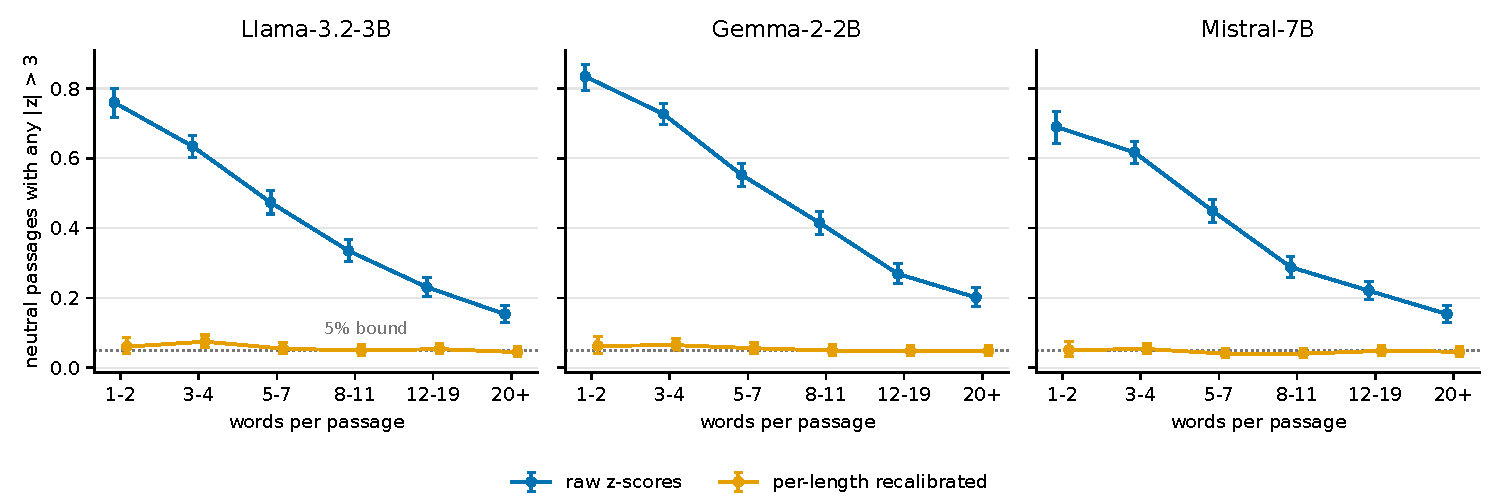
\includegraphics{../figures/fig3_neutral_false_alarm.pdf}

\hypertarget{27-training-seed-robustness-t11md-t11json-in-each-models-directory}{%
\subsubsection{\texorpdfstring{2.7 Training-seed robustness
{[}\texttt{t11.md}, \texttt{t11.json} in each model\textquotesingle s
directory{]}}{2.7 Training-seed robustness {[}t11.md, t11.json in each model\textquotesingle s directory{]}}}\label{27-training-seed-robustness-t11md-t11json-in-each-models-directory}}

The intervals in 2.1--2.2 resample test items only. Over 5 training
subsamples (seeds 0--4; each draws 80\% of the LLM-written rows and 80\%
of each human-pool class; validation set fixed), the sign of probe −
TF-IDF was stable (same sign in at least 4 of 5 seeds) in all 12 model ×
test-set cells: negative in-domain (−0.122 to −0.074 across models and
seeds) and positive on every external source (+0.039 to +0.211). The
sign of probe − sentence encoder was stable in 9 of 12 cells: negative
on ISEAR and DailyDialog for all three models (−0.104 to −0.011) and on
dair for Gemma (−0.017 to −0.002); small and positive on the frozen set
for Llama and Gemma. The unstable cells are Llama on dair and Mistral on
the frozen set and on dair, where the difference is near zero, as in
2.2. The subsamples overlap heavily, so this measures sensitivity to the
composition of the training set, not independent replication.

\hypertarget{28-steering-does-a-reading-direction-write-steering_resultsmd-steering_c1_resultsmd}{%
\subsubsection{\texorpdfstring{2.8 Steering: does a reading direction
write? {[}\texttt{steering\_results.md},
\texttt{steering\_c1\_results.md}{]}}{2.8 Steering: does a reading direction write? {[}steering\_results.md, steering\_c1\_results.md{]}}}\label{28-steering-does-a-reading-direction-write-steering_resultsmd-steering_c1_resultsmd}}

Pre-registered (PLAN\_v2 T10, committed before any generation). On
Llama-3.2-3B we added a unit direction, scaled by 0.1, 0.2 or 0.4 times
the mean token-state norm (16.2), to the residual stream after block 16
at every position, and generated three-sentence texts for 40 neutral
prompts (greedy, 60 tokens; 4,120 generations). Directions: the audited
LDA probe direction for each of 7 emotions, a v1-style mean-difference
direction for each emotion, and 20 random unit directions at every
strength. The strength grid came from a fluency-only pilot (S* = 0.4;
perplexity of the steered text under the unsteered model stayed within
1.14x). The emotion expressed was labelled by a fixed zero-shot judge
(Granite-4.2-8B, local) that passed its gate on human text (macro-F1
0.648, accuracy 0.646 on the frozen GoEmotions set;
\texttt{judge\_validation.md}).

\begin{itemize}
\tightlist
\item
  \textbf{Result: not established.} The rule needed an
  emotion\textquotesingle s steered rate to exceed all 20 random
  directions\textquotesingle{} with a bootstrap interval excluding 0,
  for at least 4 of 7 emotions. \textbf{0 of 7} met it: changes in the
  judged rate of the target emotion were within ±0.075 (point estimates)
  for every probe direction at every strength, with the generation still
  fluent; the 95\% interval bounds lie between −0.150 and +0.175. Judge
  failures (266 of 4,120 unparsed) were 6--7\% in every condition.
\item
  \textbf{Post hoc, not pre-registered:} the same rule applied to the
  mean-difference directions finds joy (+0.375 {[}+0.200, +0.525{]} at
  0.4; perplexity ratio 1.40; random maximum 0.000) and anger (+0.125
  {[}+0.025, +0.225{]}) specific, 2 of 7, still below the threshold;
  love is not fluent at its effective strength. Probe minus
  mean-difference for joy at 0.4 is −0.350 {[}−0.500, −0.175{]}.
\item
  \textbf{Power.} With 40 prompts the 95\% intervals for the probe
  directions at S* = 0.4 are 0.075--0.225 wide (anger and love show no
  change at all, so their intervals are degenerate at 0). A shift of the
  size the mean-difference direction produced for joy (+0.375) would
  have been detected; a shift of up to about +0.15 (the upper bound of
  the widest interval, joy) cannot be excluded. This is a test against
  large effects; small effects are not ruled out.
\item
  \textbf{Fluency rule.} "Fluent" means a median perplexity ratio ≤ 1.5,
  fixed in the T10 pre-registration (\texttt{PLAN\_v2.md}) and applied
  identically to probe, mean-difference and random directions. The 1.14×
  figure is the largest ratio the probe directions reached at 0.4, not a
  threshold. Mean-difference joy at 0.4 (ratio 1.40) passes; love (1.57)
  and sadness (1.68) do not.
\item
  \textbf{Norm-matched is not effect-matched (post hoc diagnostic,
  \texttt{steering\_diagnostic.md}).} On cached layer-16 states, the
  unit probe direction shifts the projection onto the class
  mean-difference axis as much per unit norm as the mean-difference
  direction does (mean cosine 0.270 against 0.274; random 0.002), so the
  null is not explained by a smaller shift on the class axis. The two
  differ in where they point: the pooled states vary with sd 0.21 along
  the probe directions, 0.59 along the mean-difference directions and
  0.10 along random ones, and at 0.4 the perplexity ratio is 1.10--1.14
  for probe directions (random 1.08--1.15 in the pilot) but 1.37--1.68
  for mean-difference directions. Adding the probe direction at matched
  norm is therefore about as disruptive as a random direction, whereas
  the mean-difference direction perturbs the model far more per unit
  norm. A probe strength between 0.4 and 0.8 was not tried (the pilot
  grid had no point there, and fluency fails at 0.8 even for random
  directions), so a stronger, fluency-matched probe intervention remains
  untested.
\item
  \textbf{Relation to prior work.} On Llama the post hoc ordering
  (mean-difference directions steer, the discriminatively fitted ones do
  not) matched Marks \& Tegmark (2023), who found difference-in-means
  directions more causally implicated than other probe directions for
  truth. The Gemma replication below does not reproduce that ordering at
  matched fluency.
\item
  \textbf{Reading (Llama only):} at the norm-matched strengths tried, a
  direction that reads emotion well (LDA directions whitened to separate
  classes) did not change what the model wrote, while the plain
  difference of means did. One model, one layer, one judge, 40 neutral
  prompts that already elicit mostly positive text (unsteered judge
  labels: joy 15, neutral 19 of 40), and a modest fluent strength
  ceiling. The replication below shows this is not general.
\end{itemize}

\textbf{Replication on Gemma-2-2B (T12/C1; pre-registered in
\texttt{PLAN\_v2.md}, \texttt{a2da166}, before any Gemma generation;
harness \texttt{probekit\_steer\_c1.py}; self-test passed: steering adds
the intended vector exactly, projection 1.000, extractor fidelity
3.7e-4).} Gemma-2-2B-it (4-bit), residual stream after block 14, the
same 40 prompts, judge and rules as T10 (6,280 generations; mean token
norm 214.4). A perplexity-only pilot fixed the strengths: regime N
(norm-matched, the T10 rule, perplexity ratio ≤ 1.5) S* = 0.2, strengths
0.05, 0.1, 0.2; regime F (fluency-matched, ratio ≤ 1.3 for every tested
direction, per direction type) s\_F = 0.3 for the LDA probe directions
and 0.1 for the mean-difference directions, so strengths 0.15, 0.3 and
0.05, 0.1. Fluency breaks earlier on Gemma than on Llama (random
directions already reach ratio 1.25 at 0.4).

\begin{itemize}
\tightlist
\item
  \textbf{H7a (probe directions beat random, ≥ 4 of 7 emotions): holds,
  at the threshold.} Specifically steerable at a fluent strength: joy
  (+0.375 {[}+0.225, +0.525{]} at 0.3, perplexity ratio 1.26; random
  maximum +0.075; also at 0.1, 0.15 and 0.2), sadness (+0.250 {[}+0.100,
  +0.400{]}, ratio 1.32; random max +0.100), fear (+0.125 {[}+0.025,
  +0.250{]}, ratio 1.29) and surprise (+0.125 {[}+0.025, +0.225{]},
  ratio 1.16), all at 0.3, the largest fluent LDA strength. In regime N
  alone (post hoc split) only joy qualifies (1 of 7). Exactly 4 of 7 is
  the minimum the rule allows, three of the four rest on the single
  strength 0.3, and the intervals are wide, so this is a fragile pass;
  it still contradicts the Llama null as a general statement.
\item
  \textbf{H7b (mean-difference better than LDA at matched fluency): not
  established.} The paired difference (mean-difference at its s\_F = 0.1
  minus LDA at its s\_F = 0.3) is negative or near zero for every
  emotion (joy −0.150 {[}−0.275, −0.025{]}, sadness −0.125 {[}−0.250,
  0.000{]}, surprise −0.125 {[}−0.225, −0.025{]}, love +0.050 {[}0.000,
  +0.125{]}); no interval is above 0 (0 of 7, rule ≥ 3).
\item
  \textbf{Descriptive (post hoc rule applied to mean-difference
  directions):} specifically steerable for joy, sadness, fear, anger and
  love (5 of 7) at 0.05--0.2, i.e. with about 3 times less norm than the
  probe directions, but fluency (ratio up to 1.44 at 0.2) limits how far
  they can be pushed. Mean-difference joy is specific in both regimes,
  anger only in regime N.
\item
  \textbf{Effect per unit norm (post hoc diagnostic,
  \texttt{steering\_c1\_diagnostic.md}):} as on Llama, the two direction
  types move the class mean-difference axis equally per unit norm (mean
  cosine 0.266 probe, 0.290 mean-difference, −0.003 random), and the
  states vary far more along the mean-difference directions (sd 7.68
  against 2.46 for the probe and 1.27 for random). In the pilot the
  mean-difference joy direction cost more fluency at the same strength
  (ratio 1.47 against 1.13 at 0.2).
\item
  \textbf{Judge:} 872 of 6,280 labels unparsed (13.9\%; 8 of 40
  unsteered), spread across conditions (probe 9--16\%, random 11--18\%
  per strength); unsteered labels: joy 17, neutral 8, sadness 3,
  surprise 3, fear 1.
\item
  \textbf{Llama fluency-matched follow-up (T13/C1b; pre-registered in
  85e7e53; \texttt{steering\_c1b\_results.md}).} Same model, layer,
  prompts, directions and judge as T10; fluency pilot on grid 0.1--0.8:
  s\_F = 0.4 (probe) and 0.3 (mean-difference), strengths \{0.2, 0.4\}
  and \{0.15, 0.3\}. H8a: probe directions specifically steerable for 0
  of 7 emotions (not established). H8b: paired mean-difference minus
  probe interval above 0 for joy (+0.275 {[}+0.125, +0.425{]}) and
  sadness (+0.150 {[}+0.050, +0.275{]}) only, 2 of 7 (3 needed; not
  established). Mean-difference directions are specific for joy (+0.350
  {[}+0.175, +0.525{]} at 0.3, perplexity ratio 1.24) and sadness
  (+0.175 {[}+0.075, +0.300{]} at 0.3, ratio 1.28). The probe arm
  largely repeats T10 conditions, which a deterministic decoder
  reproduces. Unparsed judge labels: 1/40 unsteered, 6\% for probe,
  5--6\% for mean-difference and 7--8\% for random directions.
\item
  \textbf{Estimator and training corpus are confounded (limitation of
  H7b and H8b).} The LDA probe directions were fitted on the merged2
  training set (with nuisance removal and shrinkage); the
  mean-difference directions were fitted on the lexically solvable v1
  corpus without nuisance removal. A difference between them mixes
  estimator with training data, so "mean-difference versus LDA" here
  does not isolate the estimator; a run with both fitted on the same
  data (T14/C3; below) was added to separate them.
\item
  \textbf{Same-data check on Gemma (T14/C3; pre-registered in
  \texttt{PLAN\_v2.md}, \texttt{f4cabfe};
  \texttt{steering\_c3\_results.md}).} Mean-difference directions
  refitted on the merged2 TRAIN states used for the LDA directions
  (cosine with the LDA directions 0.43--0.59). Rule H9: at least 3 of 7
  paired intervals (md-same minus LDA at matched fluency) above 0, and
  md-same specifically steerable for at least 2 of them. Result: 0 of 7
  intervals above 0, so \textbf{H9 is not established}; with the same
  training data, mean-difference directions are not better than LDA
  ones. The earlier descriptive advantage of mean-difference directions
  therefore cannot be attributed to the estimator on this model (it may
  reflect the training corpus), and the Llama contrast remains
  confounded. The LDA, random and unsteered generations of T12 were
  reused rather than regenerated (greedy decoding makes them identical);
  only the mean-difference arm and its fluency pilot were new. Judge
  unparsed labels: 869 of 6,280.
\item
  \textbf{Reading across the two models.} A direction fitted to read
  emotion can also write it, but whether it does at a fluent strength
  depends on the model and on how far one can push before fluency
  breaks; at fluent strengths the probe directions\textquotesingle{}
  effect is modest and, at norm-matched strength on Llama, absent. We
  tested whether the Llama null was an artifact of the strength grid
  (T13/C1b, pre-registered; table above): it was not for the probe
  directions. A fluency pilot on Llama allows at most 0.4 of the
  token-state norm for every tested direction (some random direction
  already exceeds the 1.3 perplexity limit at 0.5), which
  T10\textquotesingle s grid already included, so the probe directions
  are again 0/7 (H8a not established). The mean-difference directions at
  their fluent strengths (0.15 and 0.3) are specific for joy and sadness
  (post hoc description), but beat the probe directions by a paired
  interval above 0 for only 2 of 7 emotions (H8b not established; 3
  needed). So on Llama the Gemma-style pass for probe directions does
  not appear; the difference between the two models is not explained by
  grid choice. The claim "probes are not causal handles" is not
  supported in either direction: two models, one layer each, one
  zero-shot judge, 40 prompts, interval widths up to 0.25.
\end{itemize}

\hypertarget{29-audit-of-a-published-model-written-corpus-t5_audit_trained_on_t5md-t5_audit_trained_on_merged2md}{%
\subsubsection{\texorpdfstring{2.9 Audit of a published model-written
corpus {[}\texttt{t5\_audit\_trained\_on\_t5.md},
\texttt{t5\_audit\_trained\_on\_merged2.md}{]}}{2.9 Audit of a published model-written corpus {[}t5\_audit\_trained\_on\_t5.md, t5\_audit\_trained\_on\_merged2.md{]}}}\label{29-audit-of-a-published-model-written-corpus-t5_audit_trained_on_t5md-t5_audit_trained_on_merged2md}}

We applied the audit tool to one published corpus of the kind other
emotion-vector replications train on: \texttt{ryancodrai/emotion-probes}
(CC-BY-4.0; 205,200 stories of about 140 words written by Gemini 3.1 Pro
Preview, one emotion word per story, plus 1,200 neutral stories).
Pre-registered (T5/C2, PLAN\_v2, 318cf6a) before any extraction. Seven
of our labels map to its words (joyful, sad, afraid, angry, surprised,
disgusted, loving) plus neutral; topic-disjoint split (60/20/20 topics),
2 stories per class and topic: train 960, validation 320, test 320.
Llama-3.2-3B, layer 16, one run, no layer search.

\begin{itemize}
\tightlist
\item
  \textbf{In-corpus (P1; n = 320, topic-disjoint).} Probe 0.861
  {[}0.823, 0.896{]}; TF-IDF 0.930 {[}0.901, 0.957{]}; native LR 0.953;
  bag of embeddings 0.891. TF-IDF beats the probe (−0.071 {[}−0.115,
  −0.028{]}), and the corpus is lexically solvable under the
  pre-registered rule (TF-IDF ≥ 0.90). Only 0--10\% of stories contain
  the label word itself (post hoc diagnostic: stems), so the words that
  separate classes are other cue words.
\item
  \textbf{Transfer to human text (P2).} Trained on these stories, the
  probe scores 0.236 {[}0.205, 0.265{]} on GoEmotions (n = 840), 0.286
  on dair, 0.446 on ISEAR, 0.209 on DailyDialog; all above the
  shuffle-null p95, and above TF-IDF trained on the same stories on all
  three external sources (+0.131, +0.212, +0.056) and on GoEmotions
  (+0.116). The pre-registered "transfers" claim therefore holds, at low
  absolute accuracy: the HUM-trained probe scores 0.405 (dair), 0.567
  (ISEAR), 0.343 (DailyDialog), so these stories are a weaker training
  source than human text. Native LR is better than the probe on
  GoEmotions and ISEAR (post hoc contrast in the report). The stories
  are 3--4 times longer than the GoEmotions items, so writer and length
  are confounded here.
\item
  \textbf{Writer shift (P3).} A probe trained on our merged corpus
  scores 0.544 {[}0.487, 0.594{]} on the held-out stories, against 0.861
  for a probe trained on the stories\textquotesingle{} own training
  split (difference +0.319 {[}+0.255, +0.382{]}; TF-IDF +0.539). So the
  writer-shift pattern found for LLM-written training text appears from
  the other direction too: in-corpus accuracy on a model-written corpus
  mostly measures agreement with that writer.
\item
  \textbf{Limits.} One model, one layer, one corpus and one writer
  model; 7 of its 171 labels. Absolute accuracy of the probe on human
  text should not be compared across training sets of different size.
  This audit is not evidence about the quality of any other published
  probe.
\end{itemize}

\hypertarget{3-what-this-does-and-does-not-show}{%
\subsection{3. What this does and does not
show}\label{3-what-this-does-and-does-not-show}}

\textbf{Supported:}

\begin{itemize}
\tightlist
\item
  emotion directions in mid-layer states carry information beyond a bag
  of the model\textquotesingle s own embeddings (all models, all human
  sets);
\item
  they transfer across human text domains better than a lexical
  classifier trained on the same data;
\item
  the cross-domain advantage over lexical models is shared by a frozen
  sentence encoder: the probes are no better than one trained on the
  same data (H3 not supported; the encoder is better on ISEAR and
  DailyDialog, tied on dair). The hidden states themselves carry more
  than the encoder in-domain (trained classifier − encoder +0.071 to
  +0.091, post hoc), but one direction per emotion does not extract it;
\item
  the information is linear at the chosen layer;
\item
  probes trained on one model-written corpus lose heavily on another
  writer\textquotesingle s text (+0.319 {[}+0.255, +0.382{]} for the
  probe trained on the published stories against ours, on the
  stories\textquotesingle{} held-out topics; one corpus, one model, one
  layer);
\item
  probe geometry is related to human affect norms on two of three
  models.
\end{itemize}

\textbf{Not supported:}

\begin{itemize}
\tightlist
\item
  that probes beat lexical baselines in-domain on human text (they do
  not);
\item
  that scores are comparable across lengths, or that uncalibrated scores
  separate neutral from emotional human text (they do not);
\item
  that LLM-written emotion corpora are sufficient (about 0.31 vs
  0.55--0.59 macro-F1 with human training data);
\item
  that a larger model fixes the in-domain gap (7B does not);
\item
  that probes carry more emotion information than a generic frozen
  sentence encoder (H3);
\item
  that a published model-written emotion corpus is a sufficient test or
  training set (section 2.9: lexically solvable, TF-IDF 0.930 against
  the probe\textquotesingle s 0.861; a probe trained on it reaches
  0.21--0.45 macro-F1 on human sets);
\item
  that re-fitting the neutral threshold on human neutral text fixes
  neutral detection (H5: neutral recall is restored, macro-F1 falls
  0.13--0.17 for the HUM-trained probe and 0.12--0.17 for the first-run
  probe);
\item
  that prompting or another pooling helps;
\item
  that adding a probe direction to the model\textquotesingle s
  activations changes the emotion it expresses \emph{in general}: 0 of 7
  on Llama-3.2-3B, 4 of 7 (a threshold pass at the largest fluent
  strength) on Gemma-2-2B (section 2.8); and that mean-difference
  directions steer better than probe directions at matched fluency (H7b
  and H8b not established; on Gemma also not with both fitted on the
  same data, H9).
\end{itemize}

These experiments classify \emph{input text}. They test whether probes
read the emotion expressed in a passage, which is a setting where the
text itself carries most of the signal. They do not test whether probes
reveal anything that is \emph{absent} from the text, such as an emotion
the model represents but does not express. That question needs different
designs (section 5). Nothing here supports statements about a
model\textquotesingle s feelings or internal emotional state: the probes
are linear read-outs correlated with emotion-concept text.

\hypertarget{4-limitations}{%
\subsection{4. Limitations}\label{4-limitations}}

\begin{itemize}
\tightlist
\item
  \textbf{Models.} Three small 4-bit models from three families
  (2B--7B); no larger or full-precision model.
\item
  \textbf{Data.} Human evidence comes from Reddit comments plus three
  sources of mixed provenance (machine-generated hashtag labels under
  research-only terms; an ISEAR copy whose original terms we read only
  through a 2020 capture of the provider page; utterances without
  context). GoEmotions labels are noisy. The single-label rule keeps
  items with weaker rater agreement; strict unanimity left 8--29 items
  per class.
\item
  \textbf{Comparability.} Class sets differ across sources, so macro-F1
  values are not comparable across sources.
\item
  \textbf{Blinding.} A hand-written test set we used early was
  accidentally committed to the public repository. We treat all results
  on it as non-blind and base conclusions on the frozen and external
  sets.
\item
  \textbf{Multiplicity.} We report 16--20 paired comparisons per model
  per experiment with unadjusted intervals. The ≥ 3-of-4 consistency
  rules are the guard, and some results (prompted read-out, geometry on
  Mistral) did not replicate.
\item
  \textbf{Encoder baseline.} One encoder (all-mpnet-base-v2), whose own
  training data include Reddit comments, which may favour it in-domain;
  a stronger or emotion-fine-tuned encoder could widen its lead.
\item
  \textbf{Steering.} Two models (Llama-3.2-3B at layer 16, Gemma-2-2B at
  layer 14), addition at all positions, 40 neutral prompts that already
  lean positive, one zero-shot judge (macro-F1 0.648 on human text; not
  validated on the generated text; 6.5\% and 13.9\% of labels unparsed),
  fluent-strength ceilings (0.4 and 0.3 of the token-state norm), and
  limited power (interval widths up to 0.25). The Gemma pass of H7a is
  at the minimum of the rule. Small effects are not ruled out; on Llama
  a fluency-matched run (T13/C1b) gave the same 0/7 for the probe
  directions.
\item
  \textbf{Steering confound.} In T10, T12 and T13 the probe (LDA) and
  mean-difference directions were fitted on different corpora (merged2
  training set versus the v1 corpus), so the H7b/H8b contrast mixes
  estimator and training data. The same-data check (T14, H9) removes
  this confound for Gemma only; on Llama it remains.
\item
  \textbf{Post hoc analyses} (fusion with TF-IDF, lexicon strata, alarm
  thresholds) are labelled as such where reported.
\end{itemize}

\hypertarget{5-future-work}{%
\subsection{5. Future work}\label{5-future-work}}

\begin{itemize}
\tightlist
\item
  \textbf{Information not in the text.} Use minimal pairs in which the
  target sentence is identical and only the preceding context differs;
  any lexical model is constant on the target by construction. Probe the
  assistant turn in role-play where an emotion is described but hidden
  (following the "hidden emotion" condition of Sofroniew et al., 2026).
\item
  \textbf{Causal tests.} Done for two models at one layer each (section
  2.8: Llama 0 of 7 twice, Gemma 4 of 7 at the threshold;
  mean-difference directions steer some emotions). Repeat on more models
  and layers, with the estimator and training corpus separated, add
  stronger or multi-layer interventions, and validate the judge against
  human ratings of the generated text.
\item
  \textbf{Sparse autoencoders.} Gemma Scope SAE features (Lieberum et
  al., 2024) as an alternative to supervised directions, noting that
  those SAEs were trained on the base model, not the instruction-tuned
  one.
\item
  \textbf{Scale.} Larger and full-precision models.
\end{itemize}

\hypertarget{6-reproducibility-and-compliance}{%
\subsection{6. Reproducibility and
compliance}\label{6-reproducibility-and-compliance}}

Code, tests (24 model-free synthetic test files, all passing on
2026-11-22 (19 of them also from a clean checkout on 2026-11-18)),
pre-registrations and reports are in the repository. A bundled synthetic
example runs from install to a report in one command
(\texttt{probekit-audit\ -\/-demo}; \texttt{docs/AUDIT\_QUICKSTART.md}).
\texttt{probekit\_audit.py} reproduces the headline table from cached
activations exactly (Llama probe 0.510, native LR 0.521, bag of
embeddings 0.403, TF-IDF 0.599). The T11 runs are
\texttt{probekit\_t11.py} (encoder, EmoLex, human-neutral threshold,
seeds), the post hoc analyses are \texttt{probekit\_t11\_posthoc.py} and
\texttt{probekit\_steer\_diag.py}, the Gemma steering replication is
\texttt{probekit\_steer\_c1.py}, and the figures are
\texttt{make\_figures.py}; these read only committed reports and cached
states.

Third-party data stay outside the repository and are rebuilt locally
from hash-checked manifests:

\begin{itemize}
\tightlist
\item
  GoEmotions: not stored in the repository since 2026-11-19 (only ids,
  manifests and hashes); \texttt{rebuild\_human\_data.sh} rebuilds every
  GoEmotions-derived file from the original release and checks each
  against \texttt{data/DATA\_HASHES.json} (verified byte-identical).
  Earlier commits still contain the subsets. Checked against the
  original release (2026-11-18): the \texttt{google-research} repository
  that hosts it is Apache-2.0 (top-level \texttt{LICENSE}), but the
  GoEmotions README states no separate data license, and the text is
  Reddit user content, so Reddit\textquotesingle s terms and the
  authors\textquotesingle{} rights may also apply; we use it for
  non-commercial research;
\item
  dair-ai/emotion (Saravia et al., 2018): Hub license "other"; the card
  states it "should be used for educational and research purposes only"
  (the GitHub README says the same; no license file); labels are
  machine-generated from hashtags; the tweets are subject to
  Twitter\textquotesingle s terms (checked 2026-11-20);
\item
  ISEAR (Scherer \& Wallbott, 1994): Hub copy
  \texttt{savalera/isear-from-original}, a processed version tagged
  Apache-2.0 by its uploader; the original provider\textquotesingle s
  page (Swiss Center for Affective Sciences, Geneva; read through a PDF
  capture dated 2020-02-20 kept in the JULIELab/ISEAR repository,
  because the live page returned HTTP 403) says its materials are shared
  free of charge with qualified emotion researchers for non-commercial
  research and are licensed CC BY-NC-SA 3.0, and JULIELab/ISEAR
  republishes the data under that licence; the Hub
  copy\textquotesingle s card also says it should not be used for
  commercial emotion categorization systems inferring emotions of a
  natural person (checked 2026-11-20);
\item
  DailyDialog: CC-BY-NC-SA-4.0;
\item
  NRC EmoLex and VAD lexicons: non-commercial research use, no
  redistribution; used locally and never committed.
\end{itemize}

License: The Unlicense (public domain) for our code and documents
(\texttt{LICENSE} is committed); \texttt{NOTICE.md} lists the
third-party terms that remain.

\hypertarget{acknowledgments-and-use-of-ai-tools}{%
\subsection{Acknowledgments and use of AI
tools}\label{acknowledgments-and-use-of-ai-tools}}

The author used AI assistants throughout this project and takes full
responsibility for all content. Claude (Anthropic), used through
claude.ai, served as a research advisor: it proposed the audit framing
and the baselines, helped write the pre-registered decision rules,
searched and checked related work, reviewed the results and drafts at
each stage, and drafted and edited parts of this text. Claude Code
(Anthropic) implemented the code and tests, ran the model-free analyses,
produced the reports and figures, and drafted results text from those
reports; the long model runs (extraction, generation, judging) were run
by the author on local hardware. ChatGPT (OpenAI) provided one
independent review of the study plan. The language models used as
experimental instruments (the corpus writers and the steering judge) are
described in sections 1.4 and 2.8. All AI-written text and code were
checked by the author: every number in the paper is traceable to a
committed report generated by the code, and every reference was checked
against its primary source (section 7). In line with arXiv policy, no AI
system is listed as an author.

\hypertarget{appendix-a-first-pre-registered-run-t0c-merged2-training-set}{%
\subsection{Appendix A. First pre-registered run (T0c, merged2 training
set)}\label{appendix-a-first-pre-registered-run-t0c-merged2-training-set}}

The first pre-registered run trained on the merged2 training rows
(LLM-written and human rows from the earlier human corpus) instead of
HUM. Same conclusion: TF-IDF ahead in-domain, probe ahead of the bag of
embeddings. {[}\texttt{frozen\_eval.md} in each model\textquotesingle s
directory{]}

\begin{longtable}[]{@{}llll@{}}
\toprule\noalign{}
system (GoEmotions frozen set) & Llama-3.2-3B & Gemma-2-2B &
Mistral-7B \\
\midrule\noalign{}
\endhead
\bottomrule\noalign{}
\endlastfoot
probe & 0.510 {[}0.476, 0.544{]} & 0.513 {[}0.478, 0.546{]} & 0.515
{[}0.481, 0.547{]} \\
trained classifier, same states & 0.521 & 0.537 & 0.559 \\
TF-IDF & 0.599 {[}0.564, 0.630{]} & 0.599 {[}0.564, 0.630{]} & 0.599
{[}0.564, 0.630{]} \\
bag of embeddings & 0.403 & 0.401 & 0.394 \\
\end{longtable}

Probe − TF-IDF: −0.088, −0.085, −0.083 (all intervals exclude 0). Probe
− bag of embeddings: +0.107, +0.112, +0.121 (all exclude 0). TF-IDF does
not use the model, so it is identical across models. The TF-IDF
advantage is larger on items with high rater agreement (Llama: 0.594 vs
0.749 at agreement ≥ 0.67, n=244), so label noise does not explain it.

\hypertarget{7-references}{%
\subsection{7. References}\label{7-references}}

\emph{Section A was checked against the papers\textquotesingle{} own
pages on 2026-11-18. Section B was checked on 2026-11-20: arXiv items
against the arXiv API; venues, volumes and pages against the ACL
Anthology, Crossref and arXiv comment fields; the Llama 3.2 model card
against Meta\textquotesingle s repository. Where no venue could be
confirmed the entry is given as an arXiv preprint.}

\textbf{A. Checked}

\begin{itemize}
\tightlist
\item
  Fang, T., Guibon, G., \& Buscaldi, D. (2026). Some Emotions Run
  Deeper: Layer-wise Probing and Causal Intervention in Large Language
  Models. \emph{Findings of EMNLP 2026}.
\item
  Hollowell, A. (2026). Replicating the Geometry of Emotion
  Representations in a Base Open-Weights Model. arXiv:2609.22208.
\item
  Jeong, J. (2026a). Extracting and Steering Emotion Representations in
  Small Language Models: A Methodological Comparison. arXiv:2604.04064.
\item
  Jeong, J. (2026b). Shared Emotion Geometry Across Small Language
  Models: A Cross-Architecture Study of Representation, Behavior, and
  Methodological Confounds. arXiv:2604.11050.
\item
  Mohammad, S. M. (2025). NRC VAD Lexicon v2: Norms for Valence,
  Arousal, and Dominance for over 55k English Terms. arXiv:2503.23547.
\item
  Reichman, B., Avsian, A., \& Heck, L. (2026). Emotions Where Art Thou:
  Understanding and Characterizing the Emotional Latent Space of Large
  Language Models. \emph{ICLR 2026}. arXiv:2510.22042.
\item
  Sofroniew, N., Kauvar, I., Saunders, W., Chen, R., et al. (2026).
  Emotion Concepts and their Function in a Large Language Model.
  Anthropic; arXiv:2604.07729.
\item
  van der Ben, S., Baur, R., Metz, Y., \& El-Assady, M. (2026). Where Do
  Models Find Happiness? Emotion Vectors in Open-Source LLMs. \emph{ICML
  2026 Mechanistic Interpretability Workshop}. arXiv:2606.26987.
\item
  Zhang, J., \& Zhong, L. (2025). Decoding Emotion in the Deep: A
  Systematic Study of How LLMs Represent, Retain, and Express Emotion.
  arXiv:2510.04064.
\item
  Keeman, M. (2026). Whether, Not Which: Mechanistic Interpretability
  Reveals Dissociable Affect Reception and Emotion Categorization in
  LLMs. arXiv:2603.22295 (checked 2026-11-19; abstract read).
\end{itemize}

\textbf{B. Checked (2026-11-20)}

\begin{itemize}
\tightlist
\item
  Alain, G., \& Bengio, Y. (2016). Understanding intermediate layers
  using linear classifier probes. arXiv:1610.01644 (preprint; no venue
  confirmed).
\item
  Belinkov, Y. (2022). Probing Classifiers: Promises, Shortcomings, and
  Advances. \emph{Computational Linguistics}, 48(1), 207--219.
  doi:10.1162/coli\_a\_00422; arXiv:2102.12452.
\item
  Demszky, D., Movshovitz-Attias, D., Ko, J., Cowen, A., Nemade, G., \&
  Ravi, S. (2020). GoEmotions: A Dataset of Fine-Grained Emotions.
  \emph{Proc. ACL 2020} (aclanthology.org/2020.acl-main.372);
  arXiv:2005.00547.
\item
  Gemma Team (2024). Gemma 2: Improving Open Language Models at a
  Practical Size. arXiv:2408.00118.
\item
  Hewitt, J., \& Liang, P. (2019). Designing and Interpreting Probes
  with Control Tasks. \emph{Proc. EMNLP-IJCNLP 2019}
  (aclanthology.org/D19-1275); arXiv:1909.03368.
\item
  Jiang, A. Q., et al. (2023). Mistral 7B. arXiv:2310.06825.
\item
  Li, Y., Su, H., Shen, X., Li, W., Cao, Z., \& Niu, S. (2017).
  DailyDialog: A Manually Labelled Multi-turn Dialogue Dataset.
  \emph{Proc. IJCNLP 2017} (aclanthology.org/I17-1099);
  arXiv:1710.03957.
\item
  Lieberum, T., Rajamanoharan, S., Conmy, A., Smith, L., et al. (2024).
  Gemma Scope: Open Sparse Autoencoders Everywhere All At Once on Gemma
  2. \emph{Proc. BlackboxNLP 2024}
  (aclanthology.org/2024.blackboxnlp-1.19); arXiv:2408.05147.
\item
  Marks, S., \& Tegmark, M. (2024). The Geometry of Truth: Emergent
  Linear Structure in Large Language Model Representations of True/False
  Datasets. \emph{COLM 2024} (venue from the arXiv comment field);
  arXiv:2310.06824 (first posted 2023).
\item
  Meta (2024). Llama 3.2 model card (release date Oct 24, 2024; Llama
  3.2 Community License). github.com/meta-llama/llama-models,
  \texttt{models/llama3\_2/MODEL\_CARD.md}.
\item
  Mohammad, S. M., \& Turney, P. D. (2013). Crowdsourcing a
  word--emotion association lexicon. \emph{Computational Intelligence},
  29(3), 436--465 (online 2012). doi:10.1111/j.1467-8640.2012.00460.x.
\item
  Panickssery (Rimsky), N., Gabrieli, N., Schulz, J., Tong, M.,
  Hubinger, E., \& Turner, A. M. (2024). Steering Llama 2 via
  Contrastive Activation Addition. \emph{Proc. ACL 2024}
  (aclanthology.org/2024.acl-long.828); arXiv:2312.06681 (first posted
  2023).
\item
  Reimers, N., \& Gurevych, I. (2019). Sentence-BERT: Sentence
  Embeddings using Siamese BERT-Networks. \emph{Proc. EMNLP-IJCNLP 2019}
  (aclanthology.org/D19-1410); arXiv:1908.10084.
\item
  Saravia, E., Liu, H.-C. T., Huang, Y.-H., Wu, J., \& Chen, Y.-S.
  (2018). CARER: Contextualized Affect Representations for Emotion
  Recognition. \emph{Proc. EMNLP 2018}, 3687--3697
  (aclanthology.org/D18-1404); doi:10.18653/v1/D18-1404.
\item
  Scherer, K. R., \& Wallbott, H. G. (1994). Evidence for universality
  and cultural variation of differential emotion response patterning.
  \emph{Journal of Personality and Social Psychology}, 66(2), 310--328.
  doi:10.1037/0022-3514.66.2.310.
\item
  Turner, A. M., Thiergart, L., Leech, G., Udell, D., Vazquez, J. J.,
  Mini, U., \& MacDiarmid, M. (2023). Steering Language Models With
  Activation Engineering. arXiv:2308.10248 (preprint; no venue
  confirmed).
\item
  Zou, A., Phan, L., Chen, S., et al. (2023). Representation
  Engineering: A Top-Down Approach to AI Transparency. arXiv:2310.01405.
\end{itemize}

\end{document}
